\section{Electromagnetism}


%Electromagnetism

\subsection{Spinning Compass}
\begin{itemize}
\item{Preparation Time: 1 minute}
\item{Materials: batteries or other power supply (the stronger the better), wire, switch or bulb, compass (the pin in the compass demo will do)}
\item{Procedure: Connect the wire and switch/bulb to the battery or power source so that there is a strong current running through the wire. Run the wire over the compass in a straight line. If the current is DC, the compass will turn to face a new direction. If the current is AC, the compass will spin or waver back and forth quickly.}
\item{Theory: Current in a straight wire creates a magnetic field around the wire in concentric circles. The direction of the magnetic field can be found using the first right-hand-rule. DC current produces a steady magnetic field in one direction (circular), so the magnet of the compass will align itself with the field. AC current produces a constantly shifting magnetic field, so the compass will spin, trying to align itself as the field changes direction.}
\end{itemize}


\subsection{Construction of Galvanometer}

\subsubsection*{Learning Objectives}
\begin{itemize}
\item{To construct a galvanometer}
\item{To explain the uses of a galvanometer}
\item{To explain the mode of action of a galvanometer}
\end{itemize}

\subsubsection*{Background Information}
A galvanometer uses the principle of electromagnetism to detect the presence of electric current. Whenever there is a flow of current in a wire conductor, magnetic fields are created around it. The magnetic fields produced are perpendicular to the direction of current and concentric around the current itself. For this reason, a coil produces a strong magnetic field through its center, and a magnet suspended in that coil will pivot to show the direction of the magnetic field. A suspended magnet, when not placed in another field, will always face in the direction of the earth's magnetic field.  

\subsubsection*{Materials}
Magnet; sewing needle, pin or the metal part of a syringe needle; coated copper wire or speaker wire; dry cells; water; empty water bottle; small piece paper; knife, connecting wires

\subsubsection*{Preparation Procedure}
Cut the empty water bottle so that the bottom 3 cm act as a shallow dish.

\subsubsection*{Activity Procedure}
\begin{enumerate}
\item{Instruct students to rub the pin/needle on the magnet several times in one direction without scratching it. This is magnetization by stroking and may take a minute depending on the strength of the magnet.} 
\item{Have students coil the wire around the water bottle dish about 20 times and secure it with cello tape so that it is secure.} 
\item{Use a knife or razor blade to scrape at least 2 cm of the insulating coating off of each end of the copper wire.} 
\item{Have students pour water into the dish so that it is about half full.} 
\item{Stitch the pin into a small piece of paper so that the pin is secure against one side of the paper.} 
\item{Place the pin and paper gently onto the surface of the water in the dish so that it floats. The pin will rotate on the water to point North and South because it is a magnet and is following the earth's magnetic field.} 
\item{Use connecting wires to connect the dry cells to both ends of the coiled wire. Observe the reaction of the needle.} 
\end{enumerate}

\subsubsection*{Results and Conclusions}
The needle/pin will rest pointing in the N-S direction. After connecting the dry cells, the needle/pin deflects because the magnetic field produced by the coil is stronger than the earth's field. The galvanometer detects whenever there is the flow of current in the wire.  

\subsubsection*{Clean Up Procedure}
\begin{enumerate}
\item{Pick up magnetized pin/needle, keep it in a safe place. Pour the water from the cap.} 
\item{Return all materials to their proper places}
\end{enumerate}

\subsubsection*{Discussion Questions}
\begin{enumerate}
\item{What causes the needle/pin to deflect?}
\item{Why does the pin face one direction when there is no current in the coil?}
\item{Use the Left Hand Rule to predict explain which end of the pin/needle is North and which end is South.} 
\end{enumerate}

\subsubsection*{Notes}
The stitched magnetized pin should rest parallel to the coiled wire so that it can be easy to observe the deflection. The pin will turn until its direction is perpendicular to the turns in the coil. Also, the paper on which the pin is resting will eventually sink, so you will need to replace it.  

	%Right hand Rule
	
	%Force on Current Carrying Conductor
	
\subsection{Force on a Current-Carrying Wire in a Magnetic Field}

\subsubsection*{Learning Objectives}
\begin{itemize}
\item{To observe the deflection of a current-carrying wire in a magnetic field} 
\item{To use the Left Hand Rule to predict the direction of deflection or force on a current-carrying wire in a magnetic field} 
\item{Students will be able to explain the relationship between motion, electric current and a magnetic field}
\end{itemize}

\subsubsection*{Background Information}
Electromagnetism is the relationship between three quantities: electric current, magnetic fields and motion. When two of these quantities are present and perpendicular to each other, the third quantity is created. When electric current is running perpendicular to a magnetic field, a force is produced which pushes the wire in a third perpendicular direction to the current and field. The Left Hand Rule can be used to predict the direction of force and therefore the direction that the wire will move.  

\subsubsection*{Materials}
Speaker magnet from a broken radio or speaker, thin copper wire about 20 cm long, books or other objects to use as supports, two stones, two clothes pegs, knife, connecting wire, two D-cell batteries, white paper, pen.  

\subsubsection*{Preparation Procedure}
\begin{enumerate}
\item{Rip off a small piece of paper the size of the magnet or smaller.} 
\item{Use a straight-edge to draw a grid on the paper like graph paper.} 
\item{Place the speaker magnet flat on the table so that one of the poles is facing up.} 
\item{Stack books or other solid objects to either side of the speaker magnet to the same height of the magnet.} 
\item{Scrape the ends (about 2 cm) of the copper wire so that the conductor is showing.} 
\item{Stretch the copper wire across the magnet so that it is resting on top of the books on either side but not quite touching the magnet.} 
\item{Secure the copper wire on either end with clothes pegs.} 
\item{Place stones or other heavy object on the clothes pegs so that the wire is pulled tight and cannot move easily.} 
\item{Attach connecting wires to each end of the copper wire.} 
\item{Place the paper with the grid on top of the magnet just below the copper wire.} 
\end{enumerate}

\subsubsection*{Activity Procedure}
\begin{enumerate}
\item{Position yourself directly over the copper wire and magnet so that the wire's position in relation to the grid is clearly visible.} 
\item{Connect the connecting wires to the battery terminals to start a current in the wire.} 
\item{Observe any movement by the wire.} 
\end{enumerate}

\subsubsection*{Results and Conclusions}
It can be seen that the wire is deflected to one side the current is allowed to pass through it. When the current is disconnected, the wire returns to its original position. This deflection is the result of the force on the wire which is produced by a combination of the electric current and the magnetic field.  
If the direction of current is switched, the direction of the wire's deflection is also switched.  

\subsubsection*{Clean Up Procedure}
Disconnect all wires and return all materials to their proper places.

\subsubsection*{Discussion Questions}
\begin{enumerate}
\item{Explain the the sources and directions of both the magnetic field and the electric current that are present.} 
\item{In what direction is the wire deflected when the circuit is completed?}
\item{Use the Left Hand Rule to find the direction of the magnetic field assuming that the direction of force and the direction of electric current are known.} 
\end{enumerate}

\subsubsection*{Notes}
This activity demonstrates the same concept which powers a motor, namely that an electric current running perpendicular to a magnetic field feels a perpendicular force. The deflection of the wire, while small, is observable and obviously in a direction perpendicular to both the current and magnetic field.  
If the direction of the field is known, students can use the LHR to predict the direction of motion. If the direction of the field is not knows, students can find it by observing the direction of force and then using the LHR to find the magnetic field.  
It will be seen that the wire vibrates when it first deflects. This is simply because of the sudden motion to one side, not because the current is producing a wave. However, if alternating current is used, it will be seen that the repeated back-and-forth deflection of the wire does produce a standing wave. If an AC source is available, this is a good demonstration of standing waves.  

%Electromagnetic Induction

\subsection{Mapping Induced Magnetic Field from a Coil}
\begin{itemize}
\item{Preparation Time: 15 minutes}
\item{Materials: power source, length of wire about 50 cm, bulb or switch, cardboard, scissors, iron wool}
\item{Procedure: Cut the cardboard so that a single tab about 10 cm long and 3 cm wide sticks out from the larger piece. Notch this tab every 1 cm on either side and coil the wire around the tab, keeping it in place in the notches. Connect the wire to the switch/bulb and power source so that there is a strong current in the wire. Use the iron wool to sprinkle iron filings onto the tab inside the wire coil. The filings will create a single solid line the length of the coil, spreading out at each end.@Theory: A coil of wire creates a single, strong magnetic field inside it in one direction. At the ‘poles’ (for it is indeed an electromagnet) the field spreads out again. You can use the 2nd Right Hand Rule to find the direction of the field. The filings will align themselves with the strong field inside.}
\end{itemize}

\begin{figure}[h!]
\begin{center}
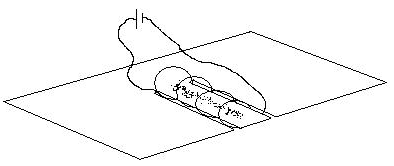
\includegraphics[width=10cm]{./img/induced-mag-field-coil.png}
\caption{Induced magnetic field in a coil}
\label{fig:induced-mag-field-coil}
\end{center}
\end{figure}

\subsection{Mapping Induced Magnetic Field from Wire}
\begin{itemize}
\item{Preparation Time: 10 minutes}
\item{Materials: power source, length of straight wire, switch or bulb, paper or cardstock, iron wool}
\item{Procedure: Cut a hole in the paper or cardstock so that the wire passes vertically through the middle of the paper so it lies flat. Connect the wire, hanging vertically, to the switch/bulb and power source so that there is a strong current in the wire. Using your thumb and forefinger, rub the iron wool to create iron filings, distributing them widely onto the paper. The filings should form concentric circles around the wire.}
\item{Theory: Current in a straight wire produces a magnetic field around the wire (use the Right Hand Rule to find the direction) in concentric circles. At the surface of the paper, the magnetic field is a series of circles and the filings will align themselves with the field.}
\end{itemize}

\begin{figure}[h!]
\begin{center}
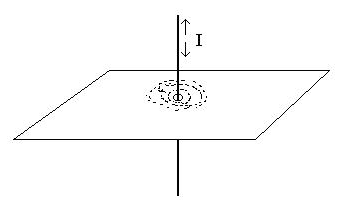
\includegraphics[width=10cm]{./img/induced-mag-field-wire.png}
\caption{Induced magnetic field in a wire}
\label{fig:induced-mag-field-wire}
\end{center}
\end{figure}

	%Lenz’s Law (direction of induced emf opposes charge that caused it)
	
\subsection{Creating a Current in a Wire}
\begin{itemize}
\item{Preparation Time: 5 minutes}
\item{Materials: Wire about 50 cm, ammeter or sensitive bulb, strong magnet}
\item{Procedure: Coil the wire to create a solenoid, connecting the free ends to the ammeter or bulb. Use a bar magnet or one pole of a horseshoe magnet and pass it through the solenoid (if you are using a speaker magnet, you will need to adjust the coil to accommodate the odd shape). As the magnet passes through the coil, the ammeter or bulb will show a current. When the magnet stops or leaves the coil, the current will cease.}
\item{Variation: If you have a very strong bar magnet, wrap the wire around a syringe multiple times and connect the ends to an ammeter. Place a small wad of cloth in the bottom of the syringe and insert the magnet. Cover the opening with your thumb and shake. The wad and your thumb will protect the magnet as it bounces back and forth, creating an alternating current in the coil.}
\item{Theory: A magnetic field that moves perpendicular to a conductor will induce a current in that conductor. When the conductor is a coil and a bar magnet is passed through it, a significant current is induced and should be enough to light a sensitive bulb or deflect the needle in an ammeter. The current will be stronger if the number of coils is increased or if a stronger magnet is used.}
\end{itemize}

	%Faraday’s Law (induced emf in mag field is prop to rate of change of mag flux)
	
	%Induction Coil 
	
	%Generators (a.c. vs. d.c., Transformers)
	
%\subsection{Simple Motor}
%
%\begin{itemize}
%\item{Preparation Time: 2 hours}
%\item{Materials: Flat piece of wood 6”x12”, four large nails, two small nails, two screws, two pieces of thick wire 4” long, rubber stopper about 1.5” diameter and at least 1” thick, 20ml syringe, two small pieces of sheet copper, lots and lots of speaker wire, hammer, knife, glue, two batteries}
%\item{Procedure:
%
%\begin{enumerate}
%\item{Arrange the piece of wood and nails/screws as follows:
%
%\begin{enumerate}
%\item{Through the center of the board, drive a large nail so that it goes all the way through; turn the board over so that the nail sticks up.}
%\item{On either side of that nail, the long way across the board, drive two other large nails into the board just enough so that they stay. The distance between these two nails should be the length of the last large nail plus about 1 cm.}
%\item{At a 45-degree angle, about 1” from the center nail and directly across from each other, drive the two small nails into the board just enough so that they stay.}
%\item{Along one long side of the board, in each corner, screw the small screws into the board, leaving a few cm between the head and the board.}
%\item{All the nails and screws are driven into the top of the board except A, which is driven up through the bottom all the way.}
%\end{enumerate}
%} % Arrange the piece of wood...
%
%\item{Electromagnets: Connect one end of a wire to the batteries. From there, wind it once around one of the screws (D) and tighten the screw to hold the wire in place. From the screw, extend the wire to the top of the nearest large nail (B) and begin winding it around the nail from the top to the bottom. More turns will produce a stronger magnet. After reaching the bottom of the magnet, extend the wire to the nearest small nail (C) and wind the wire from the bottom of the small nail to the top. At the top, solder the wire to one of the thick copper wires, called brushes. Do this again from the other terminal of the battery, to the other screw, wound down around the other large nail (B) in the same direction as the other nail, wound around the small nail to the second brush.}
%
%\item{Rotor: Remove the plunger from the syringe and cut the finger tabs off. Along the top of the syringe tube, glue the two pieces of sheet copper as shown (upside down) in figure (ii). The sheets should be about 1” wide and should each wrap around half of the syringe’s circumference, leaving about 6 mm between the strips where they meet on each side. These copper plates, together with the brushes from (2) above, form the commutator. Hollow out a small space for the syringe to fit snugly into in the bottom of the stopper. Insert the bottom of the syringe (where the needle attaches) into this space. You will glue this later, but leave it for now. Through the top of the stopper, insert the last large nail horizontally so that exactly half of the nail sticks out on either side. The nail and upside-down syringe should form a T, with the stopper at the intersection (ii). This is the armature of the rotor.}
%
%\item{Glue or solder the end of a wire to one of the copper sheets. From there, wind the wire around one half of the armature nail starting at the stopper and winding outwards. Once the wire reaches the end of the nail, extend it over to the other end of the nail on the other side of the stopper and start winding again towards the stopper, circling the opposite way around the nail (circling in the same direction will cause opposing magnetic fields – use the RHR if you get stuck on this). Once the wire reaches the stopper, extend it down to the other copper plate and glue or solder it there. You can cut the wire at this point. Put the syringe over the center large nail (A) so that it can rotate freely. The nail along the top should be able to turn, passing close to the two large nails (B). Turn the syringe in the stopper until the brushes touch the gaps between the copper plates when the armature magnet is aligned with the two upright electromagnets. The commutator and armature are now complete. Now you can glue the brushes to their respective nails so that they brush lightly against the gaps between the copper plates when the magnet is aligned.\\
%*Note: more windings will produce a stronger magnet so you can wind back and forth, but keep the same direction of the wire. Also, a syringe with a larger diameter will produce a more accurate commutator.}
%\item{The motor is now complete: allow current to run and give the armature a push to start it spinning. It may take a few tries to get it going, but if your commutator is well placed and your coils are wound in the right direction, the motor should keep going.}
%\end{enumerate}
%} % Procedure
%
%\item{Theory: The two coils on each side (B) are large electromagnets, which keep a constant polarity, as the current never changes. These coils are also connected to the thick wires, which brush against the commutator of the armature (rotating bit), so the thick wires act as the opposite battery terminals.\\
%The armature is also a large electromagnet, but as the commutator is repeatedly switching poles as it rotates and brushes against the thick wires, the direction of current, and therefore the poles of the magnet, is always switching with each half rotation.\\
%In one position with the armature magnet facing the two magnets on the side, a strong magnetic force holds it in place. As the rotor rotates (being pushed), the commutator plates switch brushes and the current through the armature reverses, thereby reversing the poles of the magnet. Now the armature magnet is attracted to the opposite upright magnet. As it passes the magnets again, 180-degrees, the current switches again and the cycle continues. As the rotor gains speed, it will become more stable.}
%\end{itemize}

% Also a pic from SnM v2 - don't use, cut this version of Simple Motor


\subsection{Simple Motor}

\subsubsection*{Learning Objectives}
\begin{itemize}
\item{To use Fleming's left-hand rule to determine the motion of the coil in the circuit} 
\item{To explain the principle of magnetic induction, which explain the motion of the rotating coil} 
\end{itemize}

\subsubsection*{Background Information}
The magnitude of the force acting on a current loop inside a magnetic field depends on the strength of the magnetic field, the amount of current flowing through the wire and the direction of the current and magnetic field.  

\subsubsection*{Materials}
Insulated copper wire, cello tape, clothes pegs, magnet, dry cells, connecting wires, two pieces of magnetic materials, switch

\subsubsection*{Preparation Procedure}
\begin{enumerate}
\item{Construct a ring of copper wire with lots of loops by wrapping the wire around any circular object with the desired diameter. Tape the coils together using cello tape so that the circular object can be removed and the ring does not fall apart. Make sure that two ends of the copper wire stick out from two opposite sides of the ring.} 
\item{ Take one end of the wire and scrape off all of the insulation coating using a razor. Take the other side and ONLY scrape off the insulation coating from half the circumference of the wire.} 
\item{Attach the two magnetic materials to two opposite sides of the speaker magnet.} 
\item{Attach the clothes pegs to the magnetic materials and suspend the coil above the magnet by placing it between the two wire loops of the pegs.} 
\item{Join the two dry cell together}
\end{enumerate}

\begin{figure}[h]
\begin{center}
\def\svgwidth{300pt}
\input{./img/simple-motor.pdf_tex}
\caption{A Simple Motor}
\label{fig:simple-motor}
\end{center}
\end{figure}

\subsubsection*{Activity Procedure}
\begin{enumerate}
\item{Connect the coils of the pegs to the terminals of the battery through the switch using the connecting wires.} 
\item{Close the switch to observe the effects}
\end{enumerate}

\subsubsection*{Results and Conclusions}
When the switch is on, the magnetic field applies a force to the current carrying wire following Fleming's left-hand rule and causes the loop to spin. If the current is increased the coil spins faster showing the force is proportional to the current. If the current is reversed the coil will rotate in the other direction, this is apparent from Flemming's left hand rule. If there is a stronger magnet the coil spins faster which shows the force is proportional to the magnetic field strength. If the insulation is left on the current from the battery can not flow into the wire so there will be no spinning. If all of the insulation is scratched off from both sides then the loop will not spin but will instead reach an equilibrium position where the force acting on the top and bottom of the loop are balanced.  

\subsubsection*{Clean Up Procedure}
Disconnect the components and keep them in their proper places.

\subsubsection*{Discussion Question}
Explain the motion of the coil of current in the magnetic field. What happens when the current in wire is increased? What happens when the current is reversed in the coil? What happens when if we use a stronger magnet? What would happen if we did not scrape off the insulation coating? What would happen if we scraped off all of the insulation coating on both sides?

\subsubsection*{Notes}
During the preparation of a commutator, on one end scratch around the whole wire, but on the other end only half the circumference should be scratched
Magnet must be pretty strong to have an obvious effect. Make the coil with as many turns as possible. 



\subsection{Inverter: Converting DC to AC} % Electricity???

\subsubsection*{Learning Objectives}
\begin{itemize}
\item{To explain the difference between Alternating Current and Direct Current} 
\item{To understand how to convert Direct Current to Alternating Current by changing the directing of current through a bulb or galvanometer} 
\item{To observe the effect of alternating current on a bulb or galvanometer} 
\end{itemize}

\subsubsection*{Background Information}
Direct Current is the current produced by any battery, cell or generator. It is current which moves in one direction only through a circuit. Alternating current is the current used in a house, school, etc. to power appliances, charge batteries, etc. It is current which changes direction many times per second; in Tanzania that current changes direction 80 times per second, so we say that the Tanzanian electrical system runs on 80 Hz, or 80 cycles per second.  
Rectifiers are used to convert AC to DC, but to convert the other way we need an inverter which can change the direction of electric current many times per second. The easiest way to do this is to switch the terminals of the battery repeatedly.  

\subsubsection*{Materials}
Four (4) dry cells in the plastic wrapping, Aluminium outer coating of a dead dry cell, thin cardboard, super glue, soldering iron and flux, several small nails or screws, connecting wires, board at least 1 ft long, bulb or galvanometer, scissors, knife, retort stand with clip or alternative, small motor, horizontal pulley, rubber band, pliers, multimeter


\subsubsection*{Preparation Procedure}
\begin{enumerate}
\item{Collect all of the necessary supplies.} 
\item{Attach the horizontal pulley near one end of the board so that it is free to rotate horizontally.} 
\item{Attach the small motor to the board so that it is also free to rotate horizontally.} 
\item{Attach the rubber band to the motor and pulley so that when the motor turns, the pulley also turns.} 
\item{Connect two connecting wires to the terminals of the motor and make sure it works by connecting two dry cells.} 
\item{On one of the dry cell packs, cut away the plastic around each of the terminals on both batteries so that the batteries can be used without removing them from the plastic.} 
\item{Solder or glue a connecting wire from the positive terminal of one of the batteries in the plastic to the negative terminal of the other battery. If needed, glue the wire down to the plastic in the middle so that it does not stick up.} 
\item{Glue the center battery pack on its side to the center of the horizontal pulley so that when the pulley turns, the battery pack turns on its side also.} 
\item{Cut a small piece of thin cardboard to fit over the battery pack (about 5 cm square).} 
\item{Glue the thin cardboard to the top of the battery pack.} 
\item{Find the exact center of rotation of the battery pack and pulley by rotating the pulley and marking the center of rotation on the cardboard with a pen.} 
\item{Remove the aluminium from the outside of a dead dry cell.} 
\item{Break the aluminium into 2 equal pieces (about 5 cm x 3 cm) by bending it with straight pliers.} 
\item{Glue the aluminium pieces to the cardboard so that there is a small space between them (so electricity cannot pass) and the hole marking the center of rotation can be seen between them.} 
\item{Rotate the pulley again to make sure that, as it rotates, the metal plates are rotating about the axis.} 
\item{Solder or glue a connecting wire from the free end of one of the batteries in the battery pack to one of the aluminium plates. Be sure that the wire is short enough that it does not stick up or out too much.} 
\item{Repeat this step for the other free battery terminal and the other aluminium plate.} 
\item{Use a multimeter to make sure that all of the wire connections are complete and that the circuit can conduct from one plate through the battery pack to the other plate. Note that the circuit is not complete because of the thin gap between the metal plates (otherwise you will have a short).} 
\item{Cut a piece of thin cardboard about 10 cm long and 4 cm wide.} 
\item{Fold the cardboard in half the long way.} 
\item{Cut two very small holes in the center of the folded edge about 2 cm apart.} 
\item{Insert connecting wires into each of these holes so that each sticks out of the folded end by about 2 cm.} 
\item{Remove the insulating from these connecting wires so that the copper ends form brush shapes and are free to bend slightly.} 
\item{Extend the connecting wires back to a bulb or galvanometer and solder or glue the ends to the terminals.} 
\item{Check that this circuit works with a multimeter or by connecting 2 dry cells across the brush ends.} 
\item{If possible, connect a switch to the bulb or galvanometer.} 
\item{Suspend the bulb/brush circuit about the rotating metal plates so that the wire brushes just touch the metal plates. If each brush is touching a different plate, the bulb or galvanometer should indicate a current.} 
\end{enumerate}

\begin{figure}
\begin{center}
\def\svgwidth{250pt}
\input{./img/inverter.pdf_tex}
\caption{An Inverter}
\label{fig:inverter}
\end{center}
\end{figure}


\subsubsection*{Activity Procedure}
\begin{enumerate}
\item{Check the circuits in the inverter by turning on the motor or touching the wire brushes to the metal plates.} 
\item{Align the wire brushes so that they rest in the thin gap between the metal plates. This will allow you to continue working or discussing without using up the battery or bulb.} 
\item{Touch the wire brushes to opposite plates to show that a direct current is flowing and the bulb produces a steady light or the galvanometer shows a single direction of current.} 
\item{Switch the plates that the brushes are touching to show that, again, a direct current is flowing and the bulb produces a steady light or the galvanometer shows a single direction of current opposite to the one previously seen.} 
\item{Connect the motor to the batteries so that the system rotates under the brushes.} 
\end{enumerate}

\begin{figure}
\begin{center}
\def\svgwidth{150pt}
\input{./img/half-wave-rectifier.pdf_tex}
\caption{A Half Wave Rectifier}
\label{fig:half-wave-rectifier}
\end{center}
\end{figure}

\begin{figure}
\begin{center}
%\def\svgwidth{250pt}
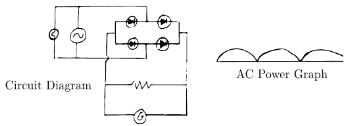
\includegraphics{./img/full-wave-rectifier.png}
\caption{A Full Wave Rectifier}
\label{fig:full-wave-rectifier}
\end{center}
\end{figure}

\subsubsection*{Results and Conclusions}
Students will see that when the metal plates are rotating under the brushes, the bulb flickers on and off quickly or the galvanometer changes direction quickly.  
Students will see that the behaviour of the bulb or galvanometer is different depending on if the plates are rotating.  
Students will understand that the bulb flickers or the galvanometer changes direction because the direction of current is changing every time the plates switch brushes.  
Students will understand that the system is converting the direct current (DC) of the battery pack to alternating current (AC) in the bulb or galvanometer.  

\subsubsection*{Clean Up Procedure}
\begin{enumerate}
\item{Disconnect the motor from the batteries and remove the bulb/brush circuit from the metal plates.} 
\item{Return all pieces to their proper places.} 
\end{enumerate}

\subsubsection*{Discussion Questions}
\begin{enumerate}
\item{What is the difference between direct and alternating current?}
\item{What is powering the bulb or galvanometer?}
\item{What is the purpose of rotating the metal plates under the wire brushes?}
\item{Why does the bulb flicker or the galvanometer repeatedly change direction when the metal plates are rotating under the wire brushes?}
\item{What type of current is powering the bulb or galvanometer when the metal plates are not rotating?}
\item{What type of current is powering the bulb or galvanometer when the plates are rotating under the brushes?}
\end{enumerate}

\subsubsection*{Notes}
Normally, alternating current changes direction 80 times per second, which we cannot see with our eyes. Therefore, the difference between AC and DC is not visible in a normal household or school electrical system. In order to see the effect of AC, we need to slow down the frequency to the point where we can see the direction changing in the galvanometer or bulb.


\subsection{Water Energy}

\subsubsection*{Learning Objectives}
\begin{itemize}
\item{To construct a simple water wheel and generator} 
\item{To explain and show the conversion of mechanical energy to electrical energy by use of a generator coil}
\item{Students will be able to show the direction of current produced by a generator}
\end{itemize}

\subsubsection*{Background Information}
Electromagnetism is the relationship between three quantities: magnetic force, electric current and motion.  When two of these quantities are present and perpendicular to each other, the third is produced.  In a motor, we use electric current in a magnetic field to produce motion: the rotation of the motor coil.  In a generator, we use motion in a magnetic field to produce electtric current.  The structure of a motor and generator are therefore almost the same.  This is the mechanism behind gas generators, wind turbines, tidal generators, and many others.

\subsubsection*{Materials}
Plastic water bottle (any size), small motor from a car stereo or other device, super glue, large nail or soldering iron, heat source, 9 water bottle caps, 8 syringe needle caps, scissors, water and pitcher, connecting wires, galvanometer.  

\subsubsection*{Hazards and Safety}
\begin{itemize}
\item{Be careful when melting the plastic pieces together.  Melted plastic can quickly cause second degree burns.  If it is easier, you can use super glue to connect the plastic pieces together.}
\end{itemize}

\subsubsection*{Preparation Procedure}
\begin{enumerate}
\item{Making the water wheel: Using a hot nail or soldering iron, melt the open end of a syringe needle cap to the side of a water bottle cap to create a sort of spoon.} 
\item{Repeat this step 7 more times to create a total of 8 identical pieces: these are the spokes and cups of the water wheel.} 
\item{Cut the top off of a water bottle just below the lip which holds the cap making sure that the edges are even.} 
\item{Melt a plastic cap over the cut end of the water bottle top so that the piece is closed on one end by the plastic bottle cap and open on the other end where a bottle cap would normally be screwed on.} 
\item{Use the hot nail or soldering iron to melt 8 holes evenly around the side of the bottle cap used in step 4. Each hole should be just wide enough to admit the thin end of a syringe needle cap; you can insert a needle cap each time you melt a hole in the bottle cap, removing the needle cap before the plastic cools.} 
\item{Insert the 8 spokes from steps 1 and 2 into the holes so that they create an 8-spoke wheel with all of the cups facing in one direction (either clockwise or anticlockwise) and at equal distances from the center.} 
\item{Melt the plastic around each spoke in the bottle cap so that they are all secure and will not come out of the center cap.} 
\item{Making the generator: Use a pin to make a small hole in the center of a plastic water bottle cap. Glue the top of the cap to the wheel of a motor so that the center of the cap and the center of the motor wheel are perfectly aligned. Note: if you have already made the wind generator, you do not need to complete these steps.} 
\item{Attach connecting wires to each terminal on the motor.} 
\item{Screw the water wheel into the motor as you would screw a bottle cap onto a bottle so that the water wheel is free to rotate about the motor's axis of rotation.} 
\end{enumerate}

\begin{figure}[h]
\begin{center}
\def\svgwidth{200pt}
\input{./img/water-turbine.pdf_tex}
\caption{Generating Electrical Current from Falling Water}
\label{fig:water-turbine}
\end{center}
\end{figure}

\subsubsection*{Activity Procedure}
\begin{enumerate}
\item{Make sure that the water wheel is free to rotate on the motor.} 
\item{Make sure that the galvanometer is working.} 
\item{Connect the wires on the generator to the terminals on the galvanometer.} 
\item{Pour water from a pitcher or spout and place the water wheel under the water so that is turns vertically.} 
\item{Observe any deflection in the galvanometer.} 
\end{enumerate}

\subsubsection*{Results and Conclusions}
Students will see that while the water wheel is turning, a current is created in the wire around the galvanometer. They should understand that the mechanical energy of the rotating wheel (or of the water falling) is being converted to electrical energy which can be read by the galvanometer. The conversion must be taking place in the motor, which they understand involves a magnetic field and a rotating coil.  

\subsubsection*{Clean Up Procedure}
\begin{enumerate}
\item{Disconnect the galvanometer and return it to its proper place.} 
\item{Unscrew the water wheel from the generator and return both to their proper places.} 
\end{enumerate}

\subsubsection*{Discussion Questions}
\begin{enumerate}
\item{What causes the water wheel to turn?}
\item{What is happening inside the motor to convert mechanical energy (rotation) into electrical energy (electric current)?}
\item{If the water wheel is turning but the galvanometer does not deflect, what are some possible causes?}
\end{enumerate}

\subsubsection*{Notes}
We convert electrical energy to mechanical energy using a motor, and we convert mechanical energy to electrical energy using a generator. In fact they are the same thing, except that the energy being put into the system is different in each case.  
For a water generator, the falling water (gravitational mechanical energy) causes the water wheel to rotate (also mechanical energy). The rotating wheel causes the wire coil in the motor to rotate. A rotating coil in a magnetic field produces an electric current in the coil, which can then be detected by the galvanometer.  

\subsection{Wind Energy}

\subsubsection*{Learning Objectives}
\begin{itemize}
\item{To explain the conversion of mechanical energy to electrical energy using a generator coil} 
\item{To construct a simple wind turbine and generator} 
\end{itemize}

\subsubsection*{Background Information}
The mechanism for the wind-powered generator is the same as that of a water-powered generator.  The force of the wind on a turbine causes the turbine to rotate.  This, in turn, causes a coil to rotate in a magnetic field, producing electric current.  These types of generators are used all over the world to produce electricity for use.

\subsubsection*{Materials}
A 1' x 1' piece of flexible plastic sheet, pin, scissors, super glue, plastic water bottle (any size) with cap, small motor from a car stereo or other device, connecting wires, galvanometer

\subsubsection*{Preparation Procedure}
\begin{enumerate}
\item{Making the propeller: Make 5 small holes in the plastic sheet: one in the middle and one at each corner.} 
\item{Cut curved lines from each side near the right-hand corner inward towards the center hole (see diagram).} 
\item{Fold each corner in towards the center so that the five holes are aligned and glue them in place.} 
\item{Remove the cap from the water bottle and cut the top of the bottle off just below the lip where the cap sits.} 
\item{Glue the water bottle top to the center of the back of the propeller so that the side of the bottle which holds the cap is facing backwards and the propeller is facing forwards.} 
\item{Making the generator: Make a small hole in the center of the bottle cap with the pin.} 
\item{Glue the top of the bottle cap to the motor wheel; use the hole to line up the center of the cap with the center of the wheel. When the motor turns, the cap should turn evenly.} 
\item{Screw the propeller into the generator as you would close the cap on a bottle. Now the propeller should be able to turn freely on the motor.} 
\item{Connect the terminals of the motor to the terminals of your galvanometer.} 
\end{enumerate}

\begin{figure}[h]
\begin{center}
\def\svgwidth{200pt}
\input{./img/wind-turbine.pdf_tex}
\caption{A Wind Generator}
\label{fig:wind-turbine}
\end{center}
\end{figure}

\subsubsection*{Activity Procedure}
\begin{enumerate}
\item{Make sure that the wind generator can turn freely and that it is connected to the galvanometer.} 
\item{Hold the propeller upright into the wind so that it spins; the galvanometer will deflect to show that a current is being created in the wire.} 
\end{enumerate}

\subsubsection*{Results and Conclusions}
When the generator and galvanometer are working and connected properly, it will be seen that as the propeller turns, a current is created in the wire causing the galvanometer to deflect. If the propeller turns just a little, the galvanometer will show a small deflection; if the propeller turns quickly, the galvanometer will show a large deflection.  
Students will observe that mechanical energy (wind) is being converted into electrical energy (electric current) using a generator. The generator uses a magnet and motion to produce an electric current, so students will see that, as with a motor, a Magnetic Field, Electric Field and Motion are related.  

\subsubsection*{Clean Up Procedure}
\begin{enumerate}
\item{Disconnect the galvanometer and connecting wires and return them to their places.} 
\item{Unscrew the propeller from the generator and return them to their places.} 
\end{enumerate}

\subsubsection*{Discussion Questions}
\begin{enumerate}
\item{Why does wind, which moves in one direction, cause the propeller to spin?}
\item{What type of energy is being used, and what type of energy is being created in this system?}
\item{What is happening in the motor to convert between the two types of energy?}
\item{If the propeller is turning but the galvanometer does not show the presence of a current, what are some possible causes?}
\end{enumerate}

\subsubsection*{Notes}
If you have constructed the water-powered generator, this activity will be very simple.  The motor used in the other generator can be used again here; simply unscrew the water wheel and replace it with the wind turbine.
